%* 
%* ------------------------------------------------------------------
%* AN02_Turnouts.tex - Application Note 02: Turnout Controls
%* Created by Robert Heller on Thu Sep 20 12:47:41 2012
%* ------------------------------------------------------------------
%* Modification History: $Log$
%* Modification History: Revision 1.1  2002/07/28 14:03:50  heller
%* Modification History: Add it copyright notice headers
%* Modification History:
%* ------------------------------------------------------------------
%* Contents:
%* ------------------------------------------------------------------
%*  
%*     Model RR System, Version 2
%*     Copyright (C) 1994,1995,2002-2012  Robert Heller D/B/A Deepwoods Software
%* 			51 Locke Hill Road
%* 			Wendell, MA 01379-9728
%* 
%*     This program is free software; you can redistribute it and/or modify
%*     it under the terms of the GNU General Public License as published by
%*     the Free Software Foundation; either version 2 of the License, or
%*     (at your option) any later version.
%* 
%*     This program is distributed in the hope that it will be useful,
%*     but WITHOUT ANY WARRANTY; without even the implied warranty of
%*     MERCHANTABILITY or FITNESS FOR A PARTICULAR PURPOSE.  See the
%*     GNU General Public License for more details.
%* 
%*     You should have received a copy of the GNU General Public License
%*     along with this program; if not, write to the Free Software
%*     Foundation, Inc., 675 Mass Ave, Cambridge, MA 02139, USA.
%* 
%*  
%* 

\chapter{Turnout Controls}
\label{chapt:Turnouts}
\typeout{$Id$}

\begin{figure}[hbpt]
\begin{centering}
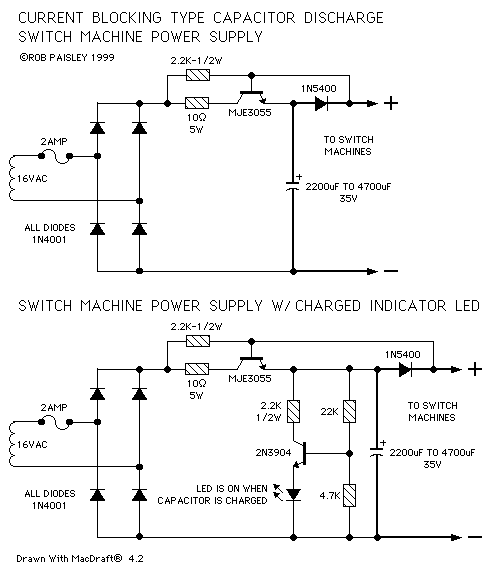
\includegraphics[width=5in]{CDblock.png}
\caption{Current Blocking Type Capacitor Discharge Switch Machine Power Supply}
\label{fig:Turnouts:CDblock}
\end{centering}
\end{figure}
\begin{figure}[hbpt]
\begin{centering}
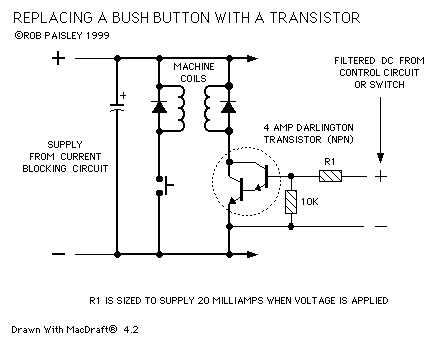
\includegraphics[width=5in]{CDtransistor.png}
\caption{Transisor control circuit}
\label{fig:Turnouts:CDtransistor}
\end{centering}
\end{figure}
\begin{figure}[hbpt]
\begin{centering}
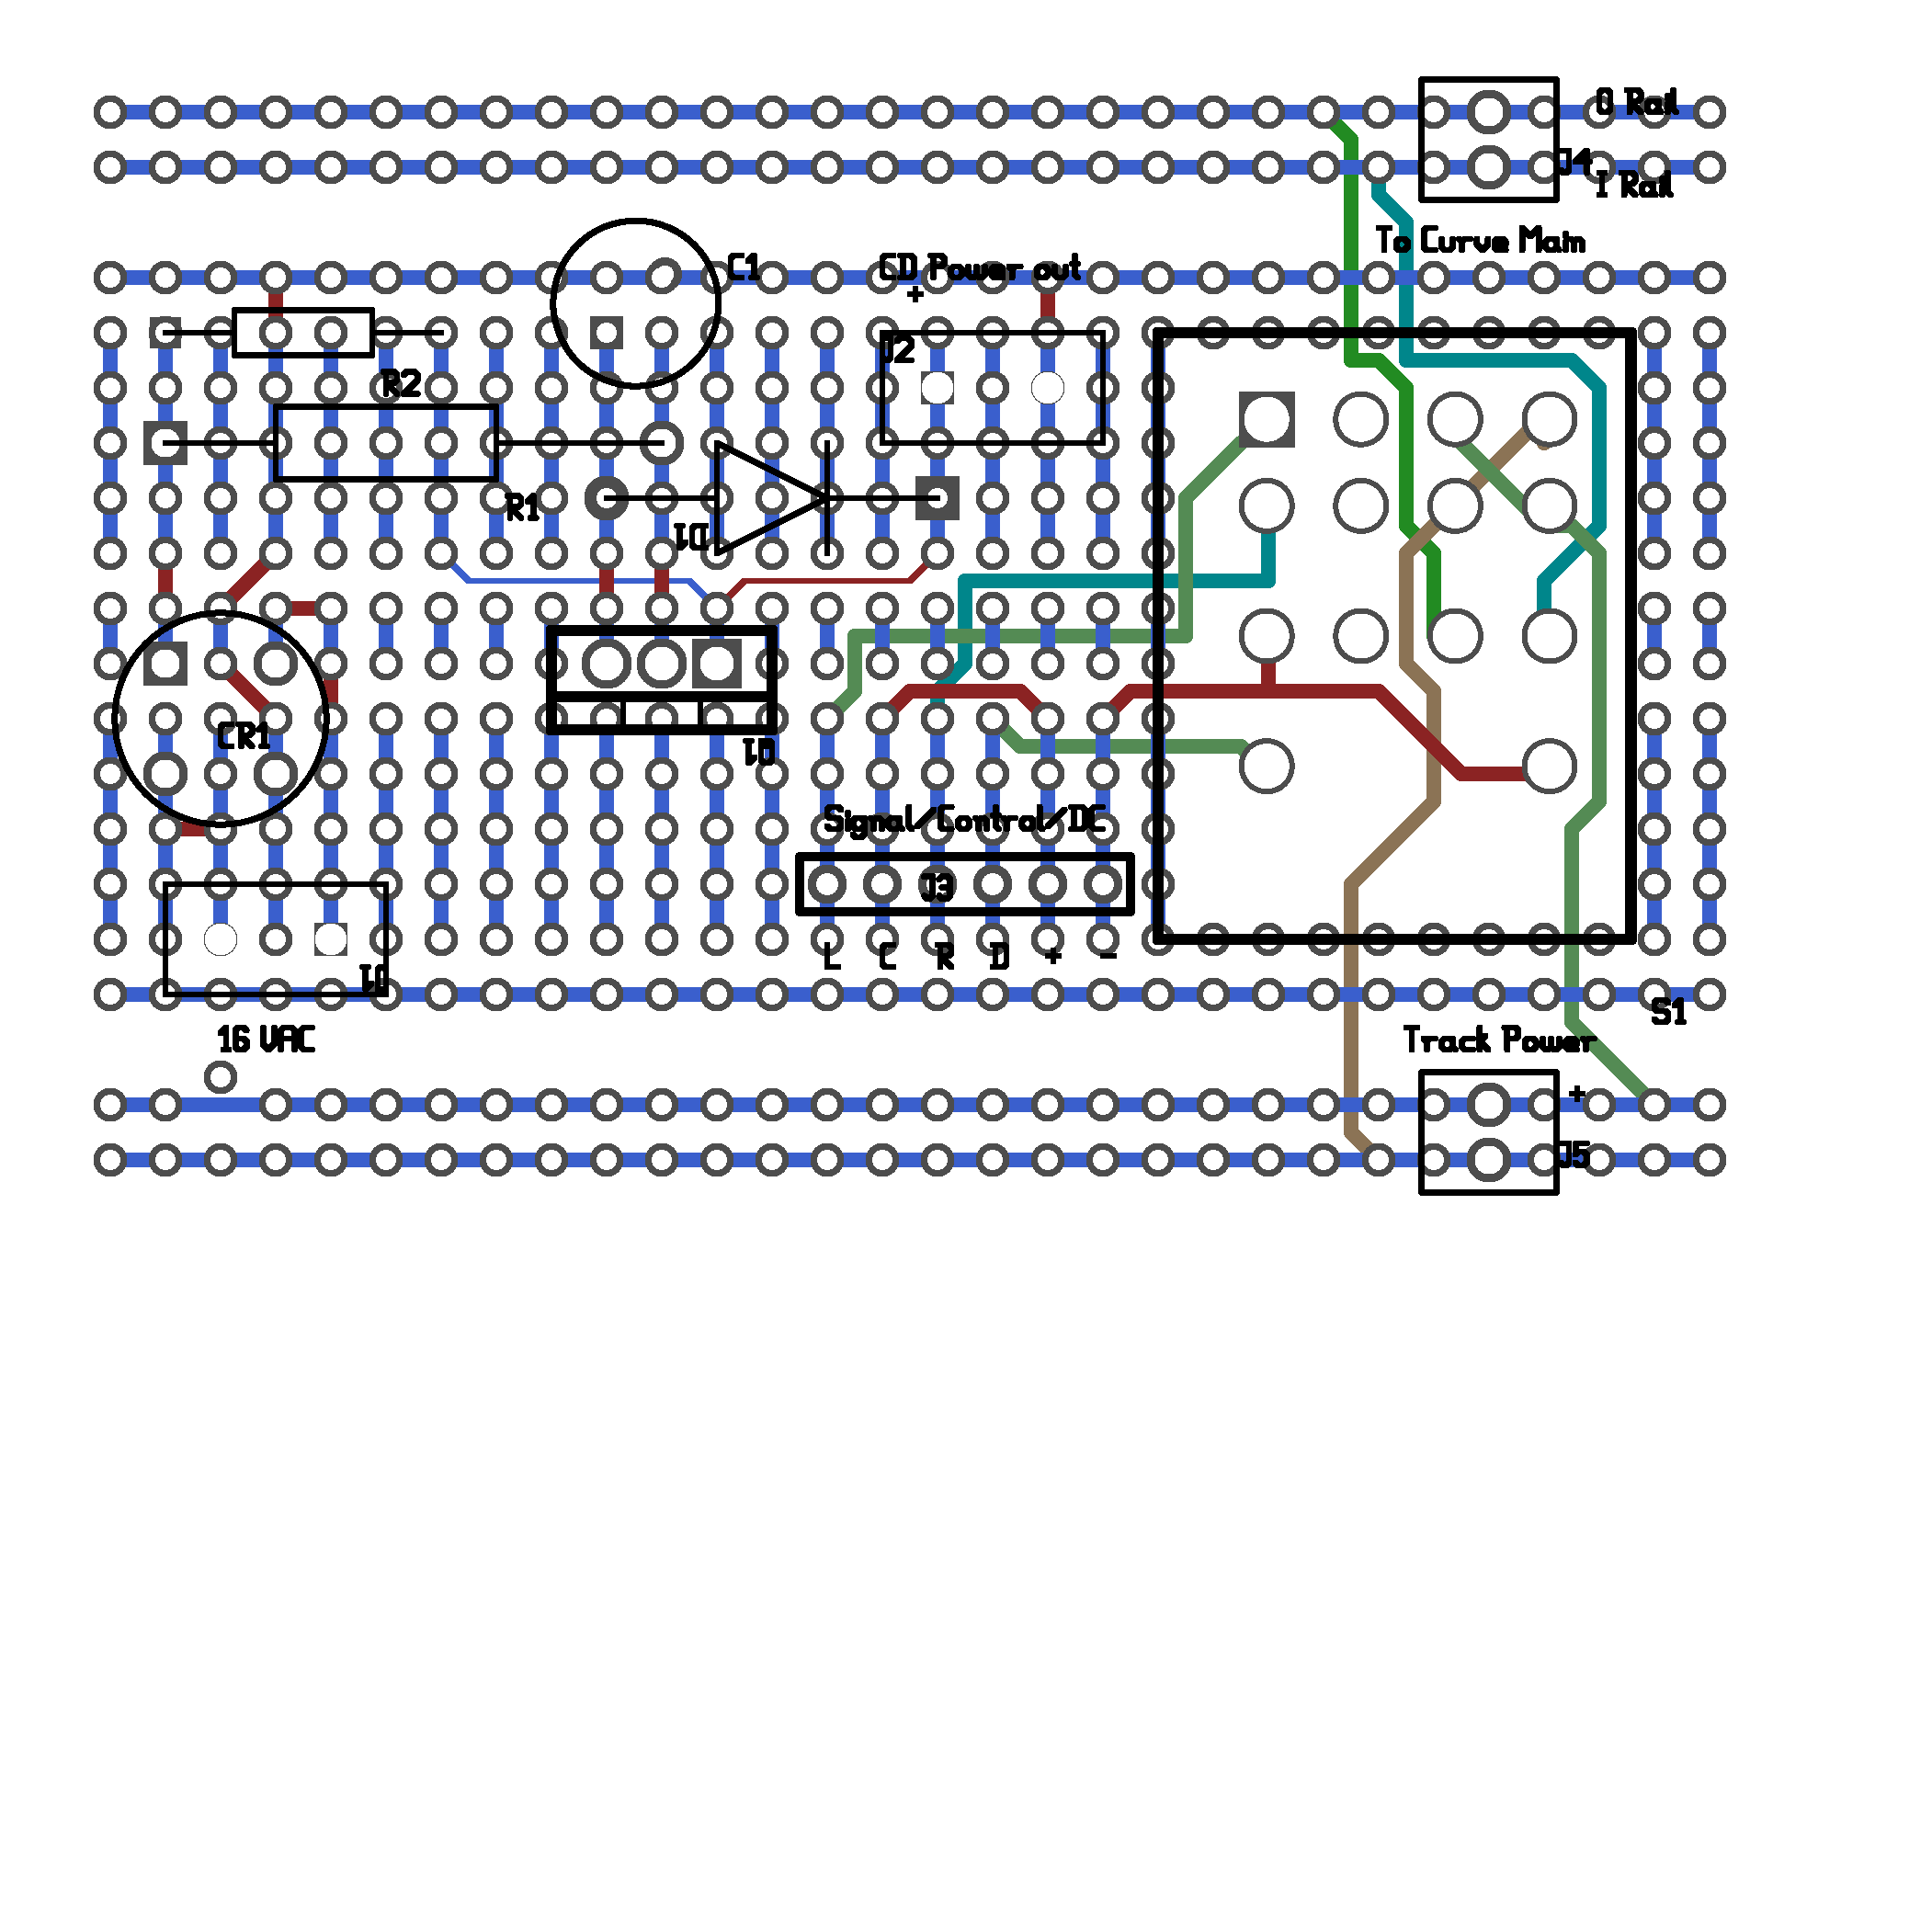
\includegraphics[width=5in]{CD-on-SB400.pdf}
\caption{Capacitor Discharge Power Supply Circuit Board}
\label{fig:Turnouts:CD-on-SB400}
\end{centering}
\end{figure}
\begin{figure}[hbpt]
\begin{centering}
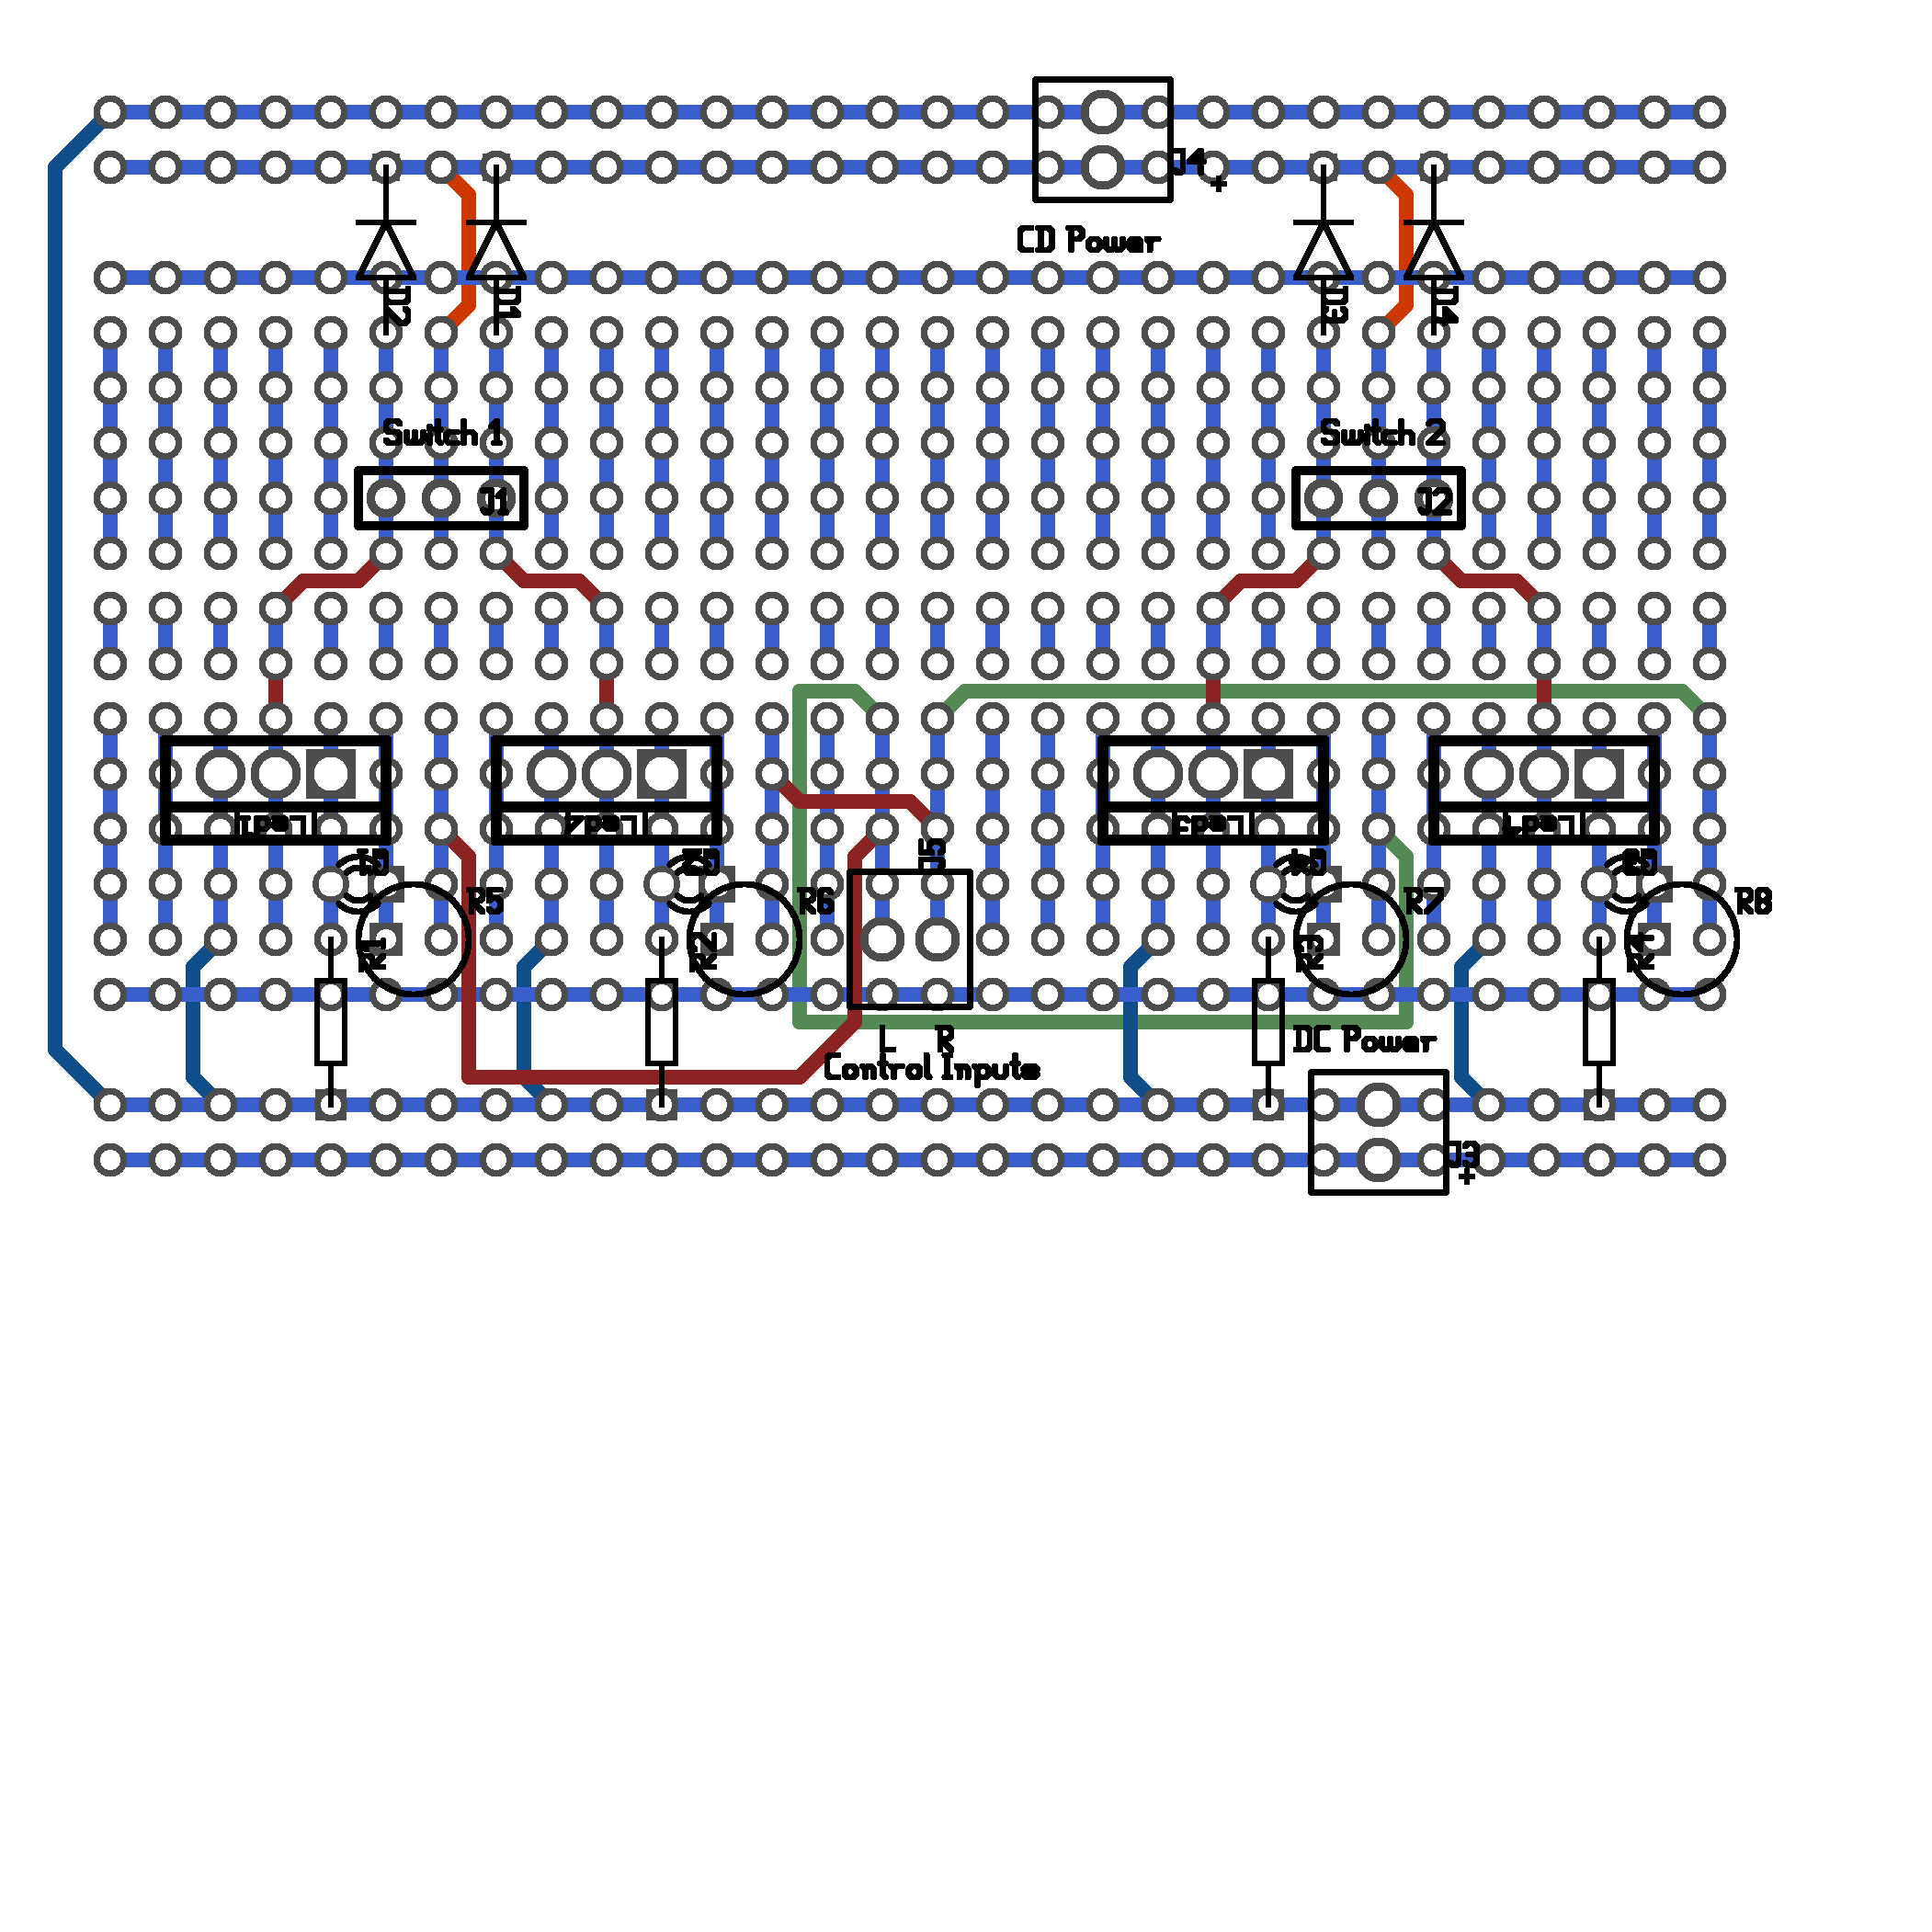
\includegraphics[width=5in]{4-CDtransistor-on-SB400.pdf}
\caption{4 transistor Switch Machine control Circuit Board}
\label{fig:Turnouts:4-CDtransistor-on-SB400}
\end{centering}
\end{figure}
The turnouts on this are controlled by twin-coil switch machines
mounted under the switches\footnote{Peco twin-coil switch machines.}.
We will be using current blocking type capacitor discharge switch
machine power supplies (Figure~\ref{fig:Turnouts:CDblock}), one for
each end of the layout, with power Darlington transistor control
circuits (Figure~\ref{fig:Turnouts:CDtransistor}).  We will build these
circuits on solderable breadboards, using circuit layouts shown in
Figures~\ref{fig:Turnouts:CD-on-SB400}\footnote{The power relay circuit
is also on this circuit board.} and \ref{fig:Turnouts:4-CDtransistor-on-SB400}. 

